\chapter*{Proposition 22}
\label{prop:22}

\begin{figure*}[ht]
    \begin{center}
    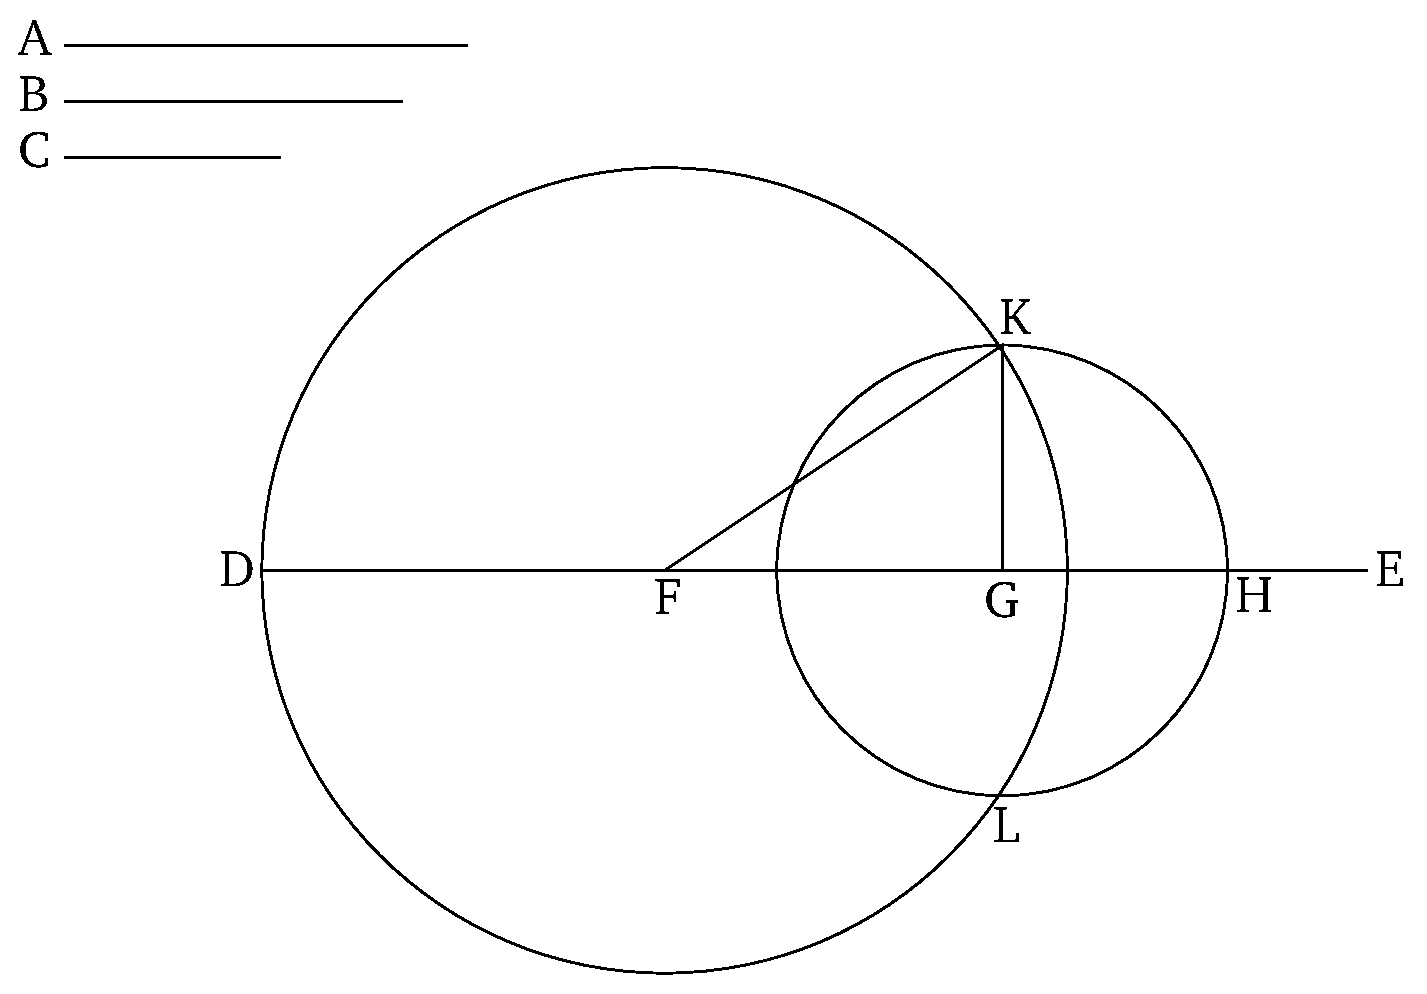
\includegraphics[width=0.5\linewidth]{figures/fig22e.eps}
    \label{fig:prop_22}
    \end{center}
\end{figure*}

To construct a triangle from three straight-lines which are equal to three given [straight-lines]. It is necessary for (the sum of) two (of the straight-lines) taken together in any (possible way) to be greater than the remaining (one), [on account of the (fact that)
 in any triangle (the sum of) two sides taken together in any (possible way) is greater than the remaining (one) [Prop.~1.20]\,].

Let $A$, $B$, and $C$ be the three given straight-lines, of which let (the sum of) two taken together in any (possible way)
be greater than the remaining (one). (Thus), (the sum of) $A$ and $B$ (is greater) than $C$, (the sum of) $A$ and $C$ than $B$,
and also (the sum of) $B$ and $C$ than $A$. So it is required to construct a triangle
from (straight-lines) equal to $A$, $B$, and $C$.

Let some straight-line $DE$ be set out, terminated at $D$, and infinite in the
direction of $E$.  And let $DF$ made equal to $A$, and $FG$
equal to $B$, and $GH$ equal to $C$ [Prop.~1.3]. And let the
circle $DKL$ have been drawn with center $F$ and radius $FD$. Again,
let the circle $KLH$ have been drawn with center $G$ and radius $GH$. And
let $KF$ and $KG$ have been joined. I say that the triangle $KFG$ has been
constructed from three straight-lines equal to $A$, $B$, and $C$.

For since point $F$ is the center of the circle $DKL$, $FD$ is equal to $FK$.
But, $FD$ is equal to $A$. Thus, $KF$ is also equal to $A$. Again, since point
$G$ is the center of the circle $LKH$, $GH$ is equal to $GK$. But, $GH$ is equal
to $C$. Thus, $KG$ is also equal to $C$. And $FG$ is also equal to $B$. Thus,
the three straight-lines $KF$, $FG$, and $GK$ are equal to $A$, $B$, and $C$ (respectively).

Thus, the triangle $KFG$ has been constructed from the three straight-lines
$KF$, $FG$, and $GK$, which are equal to the three given straight-lines
$A$, $B$, and $C$ (respectively). (Which is) the very thing it was required
to do.


\section*{Commentary}

\begin{proposition}\label{proposition_22}\lean{Elements.Book1.proposition_22}\leanok
    $A$ and $A'$ are two disctinct points on a line $AA'$. $B$ and $B'$ are two distinct points on a line $BB'$. $C$ and $C'$ are two distinct points on a line $CC'$. $|AA'| + |BB'|~>~|CC'|$, $|AA'| + |CC'|~>~|BB'|$, and $|BB'| + |CC'|~>~|AA'|$. Then, there must exist $\triangle~KFG$, s.t., $|FK| = |AA'|$, $|FG| = |BB'|$, and $|KG| = |CC'|$.
\end{proposition}
\begin{proof}
    \uses{proposition_3}\leanok
    See the original proof by Euclid.
\end{proof}


Euclid only proved that $\triangle~KFG$ can be constructed. However, in later proofs, we need $\triangle~KFG$ to be constructed on a given line and a given side of the line.

\begin{proposition}\label{proposition_22'}\lean{Elements.Book1.proposition_22'}\leanok
    $A$ and $A'$ are two disctinct points on a line $AA'$. $B$ and $B'$ are two distinct points on a line $BB'$. $C$ and $C'$ are two distinct points on a line $CC'$. $F$ and $E$ are two distinct points on a line $FE$. $|AA'| + |BB'|~>~|CC'|$, $|AA'| + |CC'|~>~|BB'|$, and $|BB'| + |CC'|~>~|AA'|$. Then, there must exist $\triangle~KFG$, s.t., $G$ and $F$ are on $FE$, $F$ not between $G$ and $E$, $|FK| = |AA'|$, $|FG| = |BB'|$, and $|KG| = |CC'|$.
\end{proposition}
\begin{proof}
    \uses{proposition_3}\leanok
    The same proof as Euclid's.
\end{proof}

\begin{proposition}\label{proposition_22''}\lean{Elements.Book1.proposition_22''}\leanok
    $A$ and $A'$ are two disctinct points on a line $AA'$. $B$ and $B'$ are two distinct points on a line $BB'$. $C$ and $C'$ are two distinct points on a line $CC'$. $F$ and $E$ are two distinct points on a line $FE$. $X$ is a point not on $FE$. $|AA'| + |BB'|~>~|CC'|$, $|AA'| + |CC'|~>~|BB'|$, and $|BB'| + |CC'|~>~|AA'|$. Then, there must exist $\triangle~KFG$, s.t., $G$ and $F$ are on $FE$, $F$ not between $G$ and $E$, $K$ on the same side of $FE$ with $X$, $|FK| = |AA'|$, $|FG| = |BB'|$, and $|KG| = |CC'|$.
\end{proposition}
\begin{proof}
    \uses{proposition_3}\leanok
    The same proof as Euclid's.
\end{proof}